\documentclass{acm}

% Pseudocode
\usepackage{amsmath}
\usepackage{algorithm}
\usepackage[noend]{algpseudocode}

\title{Tiered Log-Structured Merge Tree}
\subtitle{CS 265 Final Project, Spring '17}
\author{Jack Dent\\\email{jdent@college.harvard.edu}}

\begin{document}

\maketitle

\begin{abstract}
TODO: I present the design for a tiered Log-Structured Merge Tree (LSM Tree), as well as an implementation in C++. 
\end{abstract}

\section{Introduction}

The LSM Tree has seen increasing adoption as an industry standard for modern key-value stores, both as standalone products and as components in larger database management systems (DBMSs). Facebook's RocksDB, Google's LevelDB, and Amazon's Dynamo are prominent examples of standalone key value stores that depend on LSM Trees as their primary storage layer. SQLite4, meanwhile, dropped the B-tree in favour of the LSM Tree as the main table store. By avoiding in-place updates and instead buffering all writes in main-memory, the LSM Tree vastly improves write throughput by amortising costly roundtrips to and from secondary storage over very many write operations. When the main-memory buffer becomes full, the LSM Tree flushes its entire contents to secondary storage. On disk, the LSM Tree stores a number of levels, each of which contain a number of ``runs'' whose size increases in proportion to the level depth. To increase the performance of point and range queries, the LSM Tree stores a number of auxiliary data structures in main-memory for each run. Bloom filters allow point queries to avoid searching runs that are known to not contain the search key. Fence pointers, meanwhile, establish bounds on the run key subrange, allowing point and range queries to avoid having to read inconsequential runs into main-memory.

This paper presents the design and implementation of a parallelised LSM Tree that allows application users to control the tradeoff between read and write throughput by tuning the following parameters during initialization:

\begin{enumerate}
\item \textbf{Buffer size, $b$:} controls the number of pages in the main-memory buffer, and therefore also affects the size of runs on secondary storage.
\item \textbf{Level fanout, $f$:} controls the size ratio between the levels. All levels can contain a maximum of $f$ runs, where the maximum size of the run increases exponentially in $f$. For example, the first level contains runs of size $bf$, the second level $bf^2$, and so forth.
\item \textbf{Tree depth, $d$:} controls the number of levels on disk, and therefore the overall storage capacity of the tree.
\item \textbf{Thread count, $t$:} controls the number of worker threads dispatched to process queries in parallel.
\end{enumerate}

\section{Design}

The LSM Tree has two primary components: an in-memory buffer, and a number of ``levels'' on secondary storage of progressively increasing size. For the purposes of this paper, a ``key/value entry'' is an compact C \texttt{struct} that contains two 4-byte integers, a key and a value, and whose total size is therefore $e=8$ bytes.

\subsection{Buffer design}

The ``buffer'' is an in-memory C++ \texttt{std::set} of entry \texttt{structs}. The parameter $b$ controls the number of pages in the buffer, and the number of entries is thus given by $bp/e$, where $p$ is the size of a single page in bytes. The \texttt{std::set} data structure used in testing implemented a binary search tree and demonstrated an amortized lookup and insertion time complexity of $\Theta(\log(bp/e))$. Under most circumstances, the buffer will not be the bottleneck for workload throughput since the cost of secondary storage IO will dominate query latencies. Under workloads that exhibit highly skewed query distributions or strong time contiguity within wider distrbutions, the buffer will again become important since the majority of queries will never make it to disk. To that end, rather than attempting to optimise the buffer data structure, this project chose to focus on optimisations that applied across a broader range of workload distributions.

\subsection{Level design}

A very basic LSM Tree would store entire levels as single files containing sorted key/value entries on disk. The basic tree requires a merge/sort between the buffer and first disk level every time the buffer becomes full, and also requires that entire levels are merge/sorted when upper levels become full. Since level size increases with depth, merging two levels that potentially contain millions of entries can take a significant amount of time, during which all queries to the tree are blocked. By splitting levels into multiple runs (\textit{tiering}), the LSM Tree can reduce the complexity of the merge/sort procedure and thus improves write throughput.

% Two merge policies: controls the tradeoff between read and write performance by adjusting aggression of the merge policy between \textit{leveling} and \textit{tiering}. A \textit{leveled} LSM Tree takes a more greedy approach to merging runs by using a high value for $m$, which improves read performance by reducing the number of runs but increases the amortized write cost. A \textit{tiered} LSM Tree uses a lower value for $m$, which makes updates less costly at the expense of reads.

In my design, a ``level'' holds a time-ordered collection of ``runs'' stored in a \texttt{std::deque}. A ``run'' is an in-memory data structure that holds a pointer to a file stored on disk that stores a number of key/value entries in sorted order, a fixed-size bloom filter, and fence pointers. To mark an entry as present in the bloom filter, the LSM Tree hashes the key using three different functions and set the bit at each of the hashed positions in a bitmask to the value of 1. In case of a crash, the LSM Tree can recreate the bloom filter and the fence pointers for a run from the entries on disk, although any entries in the buffer that have not been checkpointed will be lost. Every level contains a maximum of $f$ runs at any one time, and the maximum size of each run at level $l$ (in pages) is bounded by $O(bf^l)$. A run is not guaranteed to contain the maximum number of entries, but will always contain a minimum of $\Omega(bf^{l-1})$ entries. The LSMTree never update existing runs in place.

The LSM Tree induces a global time-ordering across all runs, which fixes a pseudo-logical timestamp for each run. The global ordering is given first by level depth, and then by the position of the run within that level, where the most recent runs are stored at the front of the level \texttt{deque}. A single run will never contain more than one entry for a given key; on the other hand, there is no guarantee that different runs will not contain conflicting entries. The global ordering helps to ensure that the LSM Tree always gives preference to the most recent key/value pairing when searching and merging levels.

\subsection{PUT queries}

The LSM Tree always inserts new key/value pairs into the buffer. If the buffer is full then the store will flush the buffer to disk before attempting to insert the key. If the first level is full, in that it contains exactly $f$ runs, the store will call \texttt{MergeDown(0)} before attempting to flush the buffer to the first level. When the \texttt{MergeDown} procedure terminates (if invoked), the LSM Tree creates a new run at the start of the first level, inserts every entry in the buffer setting the relevant bloom filter entries and fence pointers, and then empties the buffer. Thus, PUT queries always create at least one new run if the buffer is full.

\subsubsection{\texttt{MergeDown} policy}

The \texttt{MergeDown($l$)} procedure for clearing space in disk levels works as follows. First, if level $l+1$ does not have space for the entries in level $l$, it recursively calls \texttt{MergeDown($i+1$)} (lines 4-5). After line 5 it is guaranteed that level $l+1$ will contain at most $f-1$ runs, and also that a run in level $l+1$ has the capacity to store all $f$ runs in level $l$. The final stage of the procedure clears level $l$ of entries, since they will now be contained by level $l+1$. The procedure then performs a merge/sort on the last $\min(mf, n_l)$ runs in level $l$ (line 5-6) and writes the results to a new run at the start of level $l+1$ (line 8). Finally, it deletes the runs that were merged from the end of level $l$ (line 9).

\begin{algorithm}
\caption{Merge down procedure}
\begin{algorithmic}[1]
\Procedure{MergeDown($l$)}{}
\State $n_l \gets \text{number of runs in level } l$
\State $n_{l+1} \gets \text{number of runs in level } l+1$
\If {$n_l < f$}
\Return
\EndIf
\If {$n_{l+1} = f$}
\State $\Call{MergeDown}{l+1}$
\EndIf
\State $r_{new} = \Call{MergeSort}{\text{runs in level } l}$
\State $\text{add } r_{new} \text{ to level } l + 1$
\State $\text{empty level } l$
\EndProcedure
\end{algorithmic}
\end{algorithm}


The parameter $m$ controls the cost of \texttt{MergeSort} operation, where $m \in \{a/f : a \in [1, f] \}$. When $m=1/f$, the \texttt{MergeDown($l$)} procedure will move at most one run between levels, whereas when $m=1$, the procedure will merge every run in the current level into a new run in the next level. Thus, a higher value of $m$ (\textit{leveling}) improves read performance at the expense of higher amortized writes costs since it enforces more ordering over the entries, whereas a lower value of $m$ (\textit{tiering}) makes writes less costly at the expense of reads.

\subsubsection{\texttt{MergeSort}}

To merge $s$ runs, the LSM Tree invokes an $s$-way external \texttt{MergeSort} procedure, which is also responsible for removing duplicates keys and pruning deleted entries from the final level. \texttt{MergeSort} pushes the first entry in each of the levels and the file pointer associated with that disk level onto a priority queue, which contains a list of $(entry, timestamp, file)$ tuples ordered first by the entry key, and second by the run timestamp. While the priority queue is not empty, the procedure pops the first tuple and writes the entry to the new run if two conditions hold:

\begin{itemize}
\item The current key is different to the last. If the current entry contains the same key as the previously seen entry, it is discarded to prevent duplicates. Since the priority queue gives precedence to runs with smaller logical timestamps in the case of key conflicts, \texttt{MergeSort} will always write the more recent entry to the new run.duplication.
\item It is not the case that the new run is in the final level and the current entry is marked as deleted. Thus, we eventually remove deleted entries from the tree.
\end{itemize}

If the file still has entries remaining, the procedure reads in the next entry and pushes the new $(entry', timestamp, file)$ tuple back onto the priority queue. Finally \texttt{MergeSort} sets the bloom filter for the new run by taking the union of the bloom filters of the previous runs, $rs$, and sets the fence pointers by taking the limit of the previous fence pointers, to remove operations from the inner merge loop: $r_{min\_key} = \min_{i \in rs} i_{min\_key}$; $r_{max\_key} = \max_{i \in rs} i_{max\_key}$; $r_{bloom\_filter} = \bigcup_{i \in rs} i_{bloom\_filter}$.

\subsubsection{Parallelisation}

A typical value for the level fanout $f$ parameter is 10, and a typical value for the merge ratio parameter $m$ is 0.5. With these parameters, each level will contain at most 10 runs, and the merge procedure will flush at most 5 runs to the next level when the current level reaches its capacity. Since this work used a machine with 4 cores to run the experiments for the LSM Tree, it therefore did not make sense to parallelise the \texttt{MergeSort} procedure.

Although this project did not experiment with larger values of $f$, the following procedure could improve the performance of PUT queries through parallelisation in those circumstances. When there are fewer than $c\cdot t$ runs to be merged at a given level, where $c$ is a tunable parameter, the LSM Tree should fall back to merging the entries in a single thread. Otherwise, the LSM Tree should uniformly partition the runs into subranges, and each thread should merge exactly one subrange, buffering the resulting array in main-memory. The main thread should wait for all of the threads to finish their merge procedures and then perform a $t$-way merge/sort over the buffers, writing the result to a new run in the appropriate level.

As an alternative, a number of (potentially preemptable) background daemon threads could proactively merge together runs in levels with low capacity.

\subsection{GET queries}

% By storing the data in each of the disk levels in sorted order, the tree can retrieve individual keys using efficient binary search. Additionally, each disk level uses a bloom filter for fast membership testing, which improves the performance of GET queries. The LSM Tree, while optimised for reads, also aims to support efficient writes by buffering incoming key/value pairs in memory before flushing them to disk in larger batches.

To search for a key, the LSM Tree first performs a lookup in the buffer. If it did not discover the key, it must then search the lower disk levels. 


Every disk level stores its key/value pairs in ascending order without duplicates, and so we implement binary search to find a key. The binary search for a given level reads in $O(\log(bf^l))$ pages, where $f$ is the tree fanout, $l$ is the level depth, and $bf^l$ is therefore the maximum number of key/value pairs in the level.

When searching a disk level, we can immediately conclude that it does not contain the specified key if any one of the three bits as the hashed positions of that key in the bitmask is 0. Since bloom filters allow false positives, we will sometimes perform an unnecessary binary search during GET queries on a given level. Importantly, however, bloom filters never return false negatives, and so we will never fail to discover a key/value pair that actually resides within a disk level.

Search the buffer. If no entry was found, then schedule the $t$ threads in the threadpool with monotonically increasing arguments in the range $[1, t]$. The argument reflects the run id, effectively acting as a timestamp for the data the thread will search. The main thread waits for all threads in the threadpool to complete and then returns the value stored in a global variable shared across all the threads (which is initially set to nullptr).

To search a run, the thread first checks the fence pointers to make sure the key is in range, and then reads the run data from disk into main memory, performing a binary search to find the value. If the thread discovered a key/value pair, and if that key/value pair is more recent than the pair discovered by all other threads to that point, it sets the value and the run id in shared memory. The thread then checks to see whether it should schedule itself again with the next lowest run id, which happens if and only if three conditions hold:

\begin{enumerate} 
  \item The value stored in global memory is still nullptr; and
  \item there are remaining runs to search. 
\end{enumerate}

The threads use a spinlock to enforce mutual exclusion around the shared memory, which contains three variables: the lowest un-searched run id, a pointer to the value variable, and a variable containing the id of the run in which the value variable was discovered.

\subsection{DELETE queries}

DELETE queries are handled almost identically to PUT queries. To delete a key, the LSM Tree inserts the key with a tombstone value. By restricting the range of possible values to $[-2147483647, 2147483647]$, it is possible to assign $-2147483648$, the minimum value of a 32 bit integer, as the tombstone. Alternatively, if we did not want to restrict the value range, we could instead increase the size of the entries stored by the tree by an additional byte, which would indicate whether the deletion status of the associated key.

We keep tombstone entries until they reach the final level. When an entry reaches the final level, it is guaranteed that there are no deeper levels containing outdated values for that key. This observation allows us to remove tombstone entries from the final level, which prevents the tree becoming saturated with deleted key/value pairings.

\subsection{RANGE queries}

I use the N-way external merge/sort procedure outlined in the PUT query to serialize every key/value pairing in the store. This is hopelessly inefficient for most small RANGE queries, and I present a plan for improving its performance in the section on parallelisation.

Stage 1 - filtering: the main thread creates an ordered queue of runs to merge/sort, where we push a run onto the queue if and only if the target range overlaps with the run's fence pointers.

Stage 2 - $t$ ($t/|Q|$)-way merge/sorts: We partition the queue into $t$ non-overlapping ordered subarrays, launch a threadpool, and assign the $i^{th}$ thread to merge/sort and filter the $i^{th}$ queue subarray into new main memory storage.

Stage 3 - $t$-way merge/sort: The main thread waits for all the threads in the threadpool to complete, and then performs a $t$ way merge/sort on the entries in the temporary main memory stores created by each thread.

\subsection{LOAD queries}

LOAD queries stream a binary file of key/value pairs, inserting each into the store in the sequence they occur. Thus, a LOAD query is almost identical to a series of independent PUT queries, with the one exception that it parses binary rather than ASCII data.

\section{Optimisations}

\subsection{Thread pool}

A ``thread pool'' is a reusable pool of kernel threads. We use a threadpool for parallelisation so that we do not have to create a new set of threads for each query. The number of threads in the threadpool is denoted $t$ and should be tuned to optimal value for the hardware, which will often be the number of cores on the machine.

\subsection{mmap}

TODO

\section{Experimental results}

Following parameters used: $b = 100$; $t = 4$; $f = 10$.

\subsection{$f$ under different workloads}

\subsection{mmap}

\subsection{Thread pool}

% \begin{figure}
% 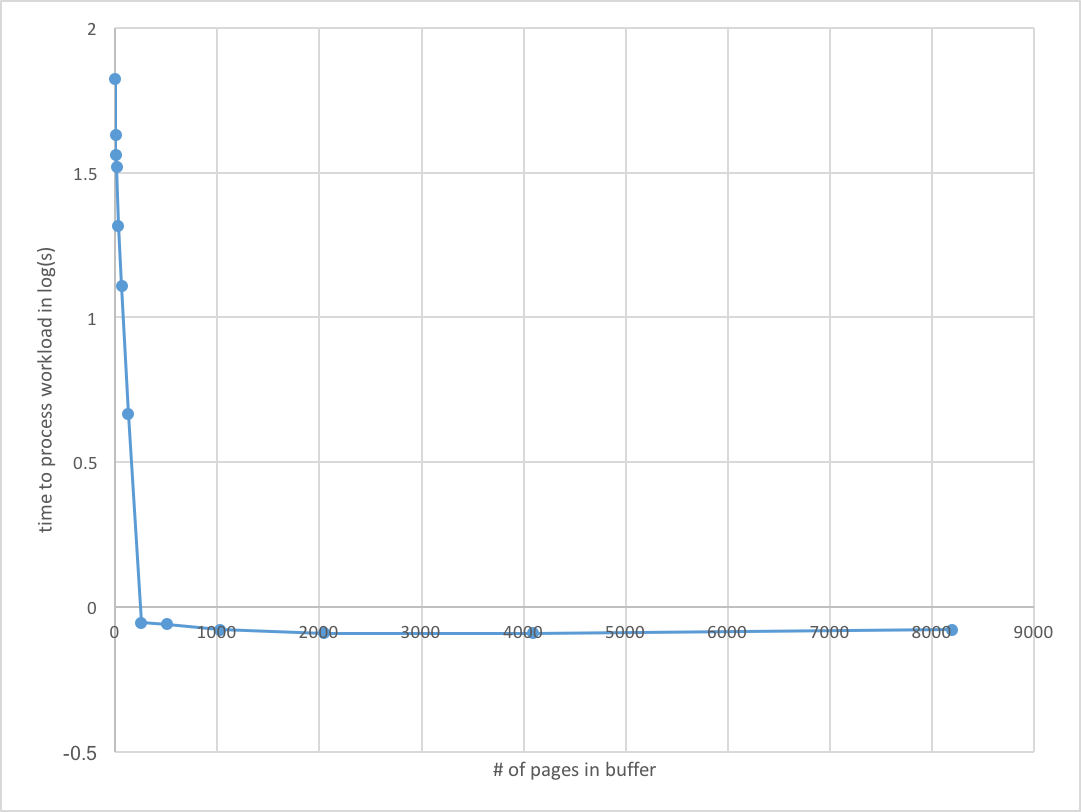
\includegraphics[width=3.3in]{chart}
% \caption{Workload latency by buffer size}
% \label{fig:example}
% \end{figure}
% Figure 1 depicts how the performance characteristics of a number of different workloads vary according to the buffer size. I tested a number of different workloads with various distrubutions for each page size, and then averaged the time taken to complete the workload. The time axis is logarithmic.

\section{Conclusion and future work}

It is unlikely that the buffer will be the performance bottleneck for the LSM Tree, but I plan to implement a skip list to improve buffer reads and writes if I have time after implementing parallelisation.

It is unlikely that the buffer will be the performance bottleneck for the LSM Tree, but I plan to implement a skip list to improve buffer reads and writes if I have time after implementing parallelisation.

Checkpointing buffer without a full cascading merge -- just persist entire buffer to disk

The size of the bloom filters is currently fixed at compile time and is equal across all levels. In the current state of the basic LSM Tree, it would be worthwile to explore two further optimisations:

\begin{enumerate}
  \item Tune the compile time parameter to find an appropriate value for expected workloads
  \item Allow the bloom filter size to vary between levels. Intuitively, levels whose size differ by an order of magnitude demand bloom filters of different size to optimise the space consumption to false positive rate.
\end{enumerate}

\end{document}
